\documentclass{beamer}
\usetheme{metropolis}
\usepackage{graphicx}
\usepackage{amsmath}
\usepackage{tcolorbox}
\title{Elementary Statistics: Math 080}
\author{Jordan Hanson}
\institute{Whittier College Department of Physics and Astronomy}

\begin{document}
\maketitle

\begin{frame}{Unit 0 Outline}
\begin{enumerate}
\item Topics from Chapter 1: 1.1, 1.2, 1.3
\begin{itemize}
\item What is a statistic?
\item Probability examples
\item Data and sampling
\end{itemize}
\item Topics from Chapter 2: 2.1 - 2.4, 2.5 - 2.8
\begin{itemize}
\item Data visualization
\item Location of the data in numerical space
\end{itemize}
\item Topics from Chapter 3: 3.1, 3.2, 3.3
\begin{itemize}
\item Two rules of probability
\end{itemize}
\end{enumerate}
\end{frame}

\section{Topics from Chapter 2}

\begin{frame}[fragile]{Stemplots}
\small
Useful for numbers like \textit{grades}. Most significant digit is the category.
\begin{table}
\begin{tabular}{| c | c |}
\hline
\hline
Stem & Leaves \\ \hline
0 &   \\ \hline
1 &   \\ \hline
2 &   \\ \hline
3 &   \\ \hline
4 & [3.0] \\ \hline
5 & [6.0] \\ \hline
6 & [7.0, 9.0] \\ \hline
7 & [8.0, 0.0, 8.0, 1.0, 2.0, 5.0, 7.0] \\ \hline
8 & [8.0, 3.0, 4.0, 6.0, 2.0, 1.0, 2.0, 1.0] \\ \hline
9 & [8.0, 7.0, 1.0, 4.0] \\ \hline
\hline
\end{tabular}
\caption{A \textit{stemplot} of a grade distribution.}
\end{table}
\end{frame}

\begin{frame}[fragile]{Stemplots}
\small
Procedure:
\begin{enumerate}
\item Identify the approximate order of magnitude of the sample.
\item Within that order of magnitude, create $\approx 10$ \textit{stems,} corresponding to the base-10 digits.
\item For each data point, call the non-most significant digits the \textit{leaves} and drop the leaves in the category with the matching leaf.
\end{enumerate}
\textbf{Professor example:} What is the stemplot of 
\begin{verbatim}
[11, 22, 33, 44, 55, 66]
\end{verbatim}
\end{frame}

\begin{frame}[fragile]{Stemplots}
\small
Procedure:
\begin{enumerate}
\item Identify the approximate order of magnitude of the sample.
\item Within that order of magnitude, create $\approx 10$ \textit{stems,} corresponding to the base-10 digits.
\item For each data point, call the non-most significant digits the \textit{leaves} and drop the leaves in the category with the matching leaf.
\end{enumerate}
Let's create a stemplot of:
\begin{enumerate}
\item Our ages in MATH080
\item My age and the rest of my department
\end{enumerate}
(Stemplots lead in to the topic of histograms)
\end{frame}

\begin{frame}[fragile]{Histograms}
\alert{Histograms} are a tool for measuring \textit{probability distributions}.  The inputs are the data points and the corresponding relative frequencies, or plain frequencies. \\ \vspace{0.5cm}
\textbf{How many textbooks or books did you purchase for school last year?} (Type in the chat).
\begin{enumerate}
\item Determine the bins, or \textit{binning}
\item For each data point, drop it into the appropriate bin
\item Each time a measurement is dropped into a bin, the \textit{count} increases by 1.
\item If a histogram displays plain frequencies, it is called \textit{un-normalized.}
\item If a histogram displays relative frequencies, it is called \textit{normalized.}
\end{enumerate}
\end{frame}

\begin{frame}[fragile]{Histograms}
\begin{enumerate}
\item Histogram of books, by hand
\item Repeat with Excel/Calc
\end{enumerate}
Practice with the FREQUENCY function in Calc/Excel:
\begin{verbatim}
=FREQUENCY(A1:A99; B1:B11)
\end{verbatim}
Then press \alert{\textbf{control+shift+enter}} to execute on arrays of data and bins.  To \textit{normalize}, input the relative frequencies, or divide frequecies by $N$.  Assume the data is in C column:
\begin{verbatim}
=C1/N ...
\end{verbatim}
\end{frame}

\begin{frame}[fragile]{Histograms}
\small
For data that is appropriately ``stationary,'' we can use histograms to estimate the mean \textit{faster}, since we only have to loop over bins rather than every data sample.  Let $H_i$ represent the counts in a given bin, and $i$ represent the bin sample.  We have:
\begin{equation}
\bar{x} = \frac{1}{N}\sum_{i=1}^{M}i H_i 
\end{equation}
To obtain the mean in signal \textit{amplitude}, you'll have to convert bin number to amplitude.  \textbf{Professor example.}
\end{frame}

\begin{frame}[fragile]{Histograms}
\small
When is a histogram appropriate?
\textbf{Note}: There is a distinction between the \textit{process or signal process} and the \textit{the data}.  Just because the data has a given $\bar{x}$ and $s$ does not imply that the signal process has or will continue to have the exact same values of $\mu$ and $\sigma$.  The underlying process could be \textit{non-stationary}.
\begin{figure}
\centering
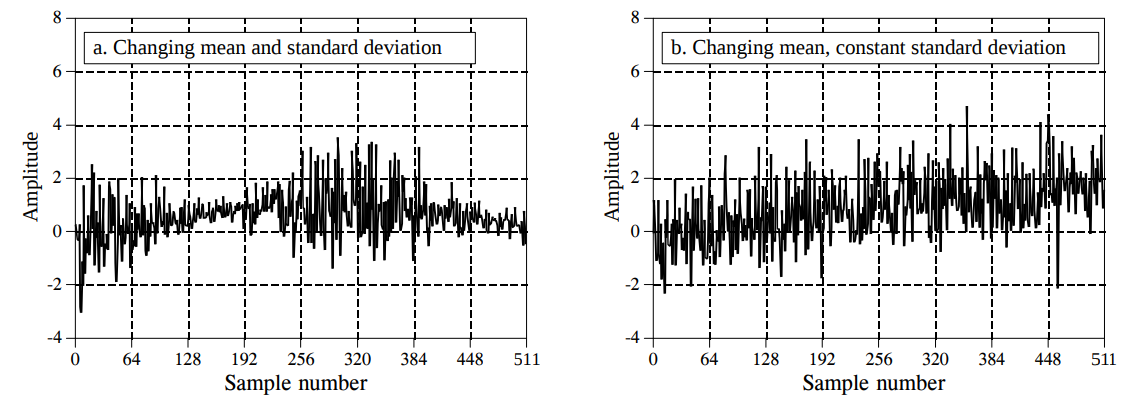
\includegraphics[width=0.9\textwidth]{figures/non_stationary.png}
\caption{\label{fig:non_stationary} Signal processes in (a) and (b) are considered \alert{non-stationary} because one or both of $\mu$ and $\sigma$ depend on time.}
\end{figure}
\end{frame}

\section{Interactive Questions}

\begin{frame}{Interactive Questions}
Which of the following pairs of number have the same \textit{stem}?
\begin{itemize}
\item A: 17 and 27
\item B: 33 and 43
\item C: 16 and 11
\item D: -1 and 1
\end{itemize}
\end{frame}

\begin{frame}{Interactive Questions}
How many \textit{leaves} are there for the stems, given the data set? \\
Data set: 67, 77, 72, 74, 90, 91, 94, 88, 82. \\
Stems: 6, 7, 8, and 9
\begin{itemize}
\item A: 1, 3, 3, 2
\item B: 1, 3, 2, 3
\item C: 1, 3, 3, 3
\item D: 1, 2, 2, 3
\end{itemize}
\end{frame}

\begin{frame}{Interactive Questions}
Consider the following relative frequencies below.  Is the corresponding histogram \textit{normalized?}\\
Relative frequencies: 0.1, 0.1, 0.25, 0.1, 0.1, 0.05
\begin{itemize}
\item A: Yes
\item B: No
\end{itemize}
\end{frame}

\begin{frame}{Interactive Questions}
What is the \textit{mean} of the histogram data below? \\
Bins: 0, 2, 4, 6, 8, 10 \\
Data: 10, 60, 20, 5, 1, 1
\begin{itemize}
\item A: 0.98
\item B: 2.56
\item A: 4.11
\item B: 10
\end{itemize}
\end{frame}

\section{More on Histograms}

\begin{frame}{More on Histograms}
\textit{\alert{Normalization} - To convert all the frequencies to relative frequencies.}
\begin{itemize}
\item Looking at fractions is helpful for \textit{relative} questions about data. (Professor example).
\item Makes calculating the mean simple, the idea of a \textit{weighted average}. (Professor example).
\item Summing a subset of bins is a \textit{probability}, not a \textit{count}. (Professor example).
\end{itemize}
\end{frame}

\begin{frame}{More on Histograms}
\begin{figure}
\centering
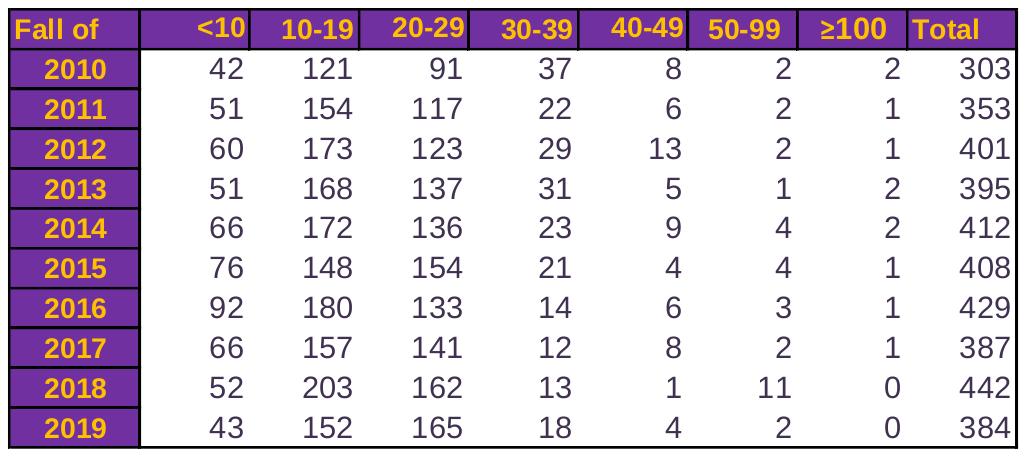
\includegraphics[width=0.8\textwidth]{figures/class_size.png}
\caption{\label{fig:class_size} A table of class sizes at Whittier College.}
\end{figure}
\end{frame}

\begin{frame}{More on Histograms}
\begin{enumerate}
\item In your notebook, create a normalized histogram of of the 50-99 column of Fig. \ref{fig:class_size}.
\item For your histogram class size, what fraction of all classes of this size come from the years 2010-2014?  What is the fraction that come from 2015 onwards?
\item What is the \textit{mean} of the histogram?
\end{enumerate}
\end{frame}

\begin{frame}{More on Histograms}
\textbf{Two-dimensional histograms.}  There's no reason to restrict to one dimension... (Professor: draw a 2D histogram of Fig. \ref{fig:class_size} below). \\ \vspace{6cm}
How do you think about the \textit{mean}?
\end{frame}

\section{More on Time-Series Data}

\begin{frame}{More on Time-Series Data}
We also think of the left-most column as \textit{time slices}, and then we can frame the rest of the data as a time-series.
\begin{figure}
\centering
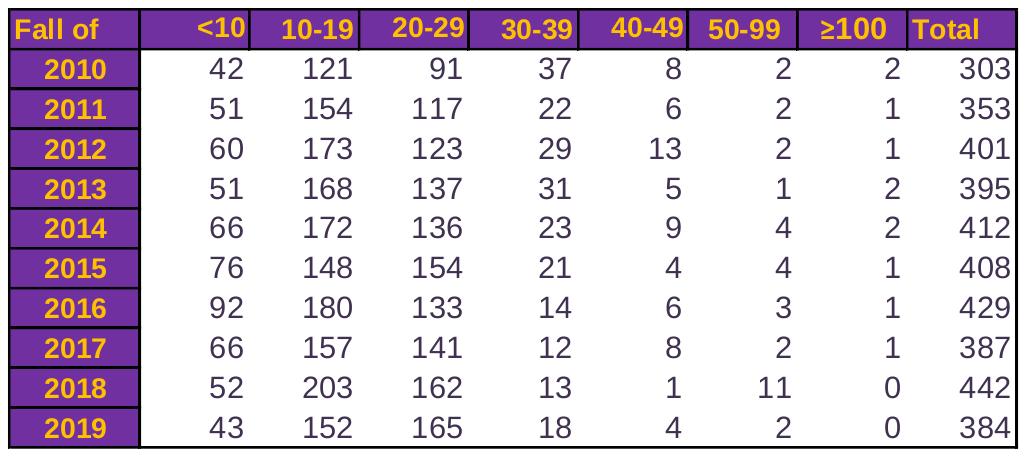
\includegraphics[width=0.8\textwidth]{figures/class_size.png}
\caption{\label{fig:class_size2} A table of class sizes at Whittier College.}
\end{figure}
\end{frame}

\begin{frame}{More on Histograms}
\textbf{Graphing time-series to look for trends.} (Make a time-series of the class-size data below). \\ \vspace{6cm}
\end{frame}

\section{Locating the Center of the Data}

\begin{frame}{Locating the Center of the Data}
\begin{enumerate}
\item \textbf{\alert{Median}} - The data value that halves a sorted list of data
\item \textbf{\alert{Mode}} - The data value with the highest frequency
\item \textbf{\alert{Mean}} - The average using either definition
\item \textbf{\alert{Quartiles}} - The values $Q_i$ that divide a sorted list into quarters of equal frequency
\item \textbf{\alert{IQR}} - $Q_3 - Q_1$
\item \textbf{\alert{k-th Percentile}} - $i = k/100 (n+1)$, where $i$ is the index of the k-th percentile, and $n$ is the number of data points in a sorted list
\item \textbf{\alert{Percentile of a value}} - (next slide)
\end{enumerate}
\end{frame}

\begin{frame}{Locating the Center of the Data}
An algorithm for finding the percentile of a particular value:
\begin{itemize}
\item Order the data from smallest to largest.
\item x = the number of data values counting from the bottom of the data list up to but not including the data value for which
you want to find the percentile.
\item y = the number of data values equal to the data value for which you want to find the percentile.
\item n = the total number of data.
\item Calculate: $(x+0.5y)/n \times 100$ and round to nearest integer.
\end{itemize}
\end{frame}

\section{The Spread of the Data}

\begin{frame}[fragile]{Statistics and Probability: The Normal Distribution}
The \textit{mean}, $\mu$, and \textit{standard deviation}, $\sigma$, of a data set $\lbrace x_i \rbrace$ are defined as
\begin{align}
\mu &= \frac{1}{N}\sum_{i=1}^N x_i \\
\sigma^2 &= \frac{1}{N-1}\sum_{i=1}^N\left(x_i-\mu\right)^2
\end{align}
Octave commands:
\begin{verbatim}
x = randn(100,1);
mean(x)
std(x)
\end{verbatim}
\end{frame}

\begin{frame}[fragile]{Statistics and Probability: The Normal Distribution}
One nice theorem: \textit{The variance is the average of the squares minus the square of the average.}  Let $\langle x \rangle$ represent the average of the quantity or expression $x$.  We have
\begin{equation}
\sigma_x^2 = \langle x^2 \rangle - \langle x \rangle^2
\end{equation}
Proof: observe on board.
\end{frame}

\begin{frame}[fragile]{Statistics and Probability: The Normal Distribution}
\small
\textbf{Note}: There is a distinction between the \textit{process or signal process} and the \textit{the data}.  Just because the data has a given $\mu$ and $\sigma$ does not imply that the signal process has or will continue to have the exact same values of $\mu$ and $\sigma$.  The underlying process could be \textit{non-stationary}.
\begin{figure}
\centering
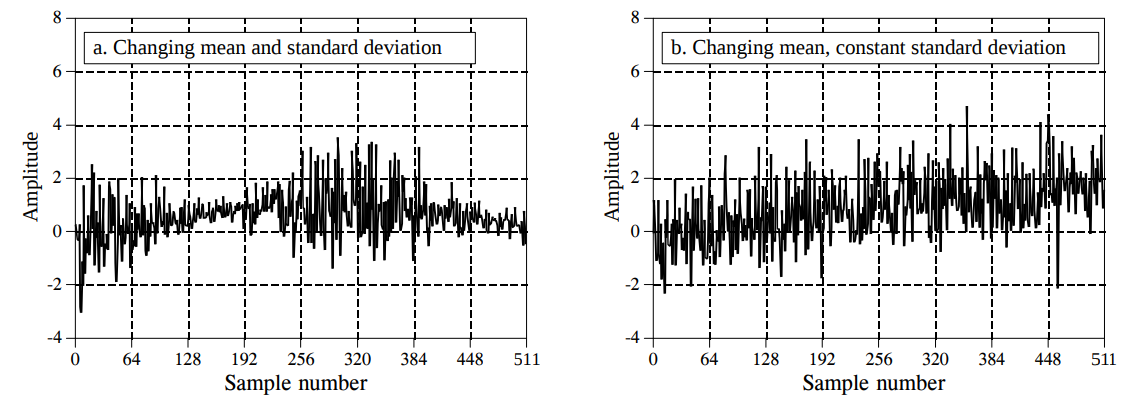
\includegraphics[width=0.9\textwidth]{figures/non_stationary.png}
\caption{\label{fig:non_stationary2} Signal processes in (a) and (b) are considered \alert{non-stationary} because one or both of $\mu$ and $\sigma$ depend on time.}
\end{figure}
\end{frame}

\begin{frame}[fragile]{Statistics and Probability: The Normal Distribution}
\small
\textbf{A histogram} is an object that represents the frequency\footnote{Careful: the word frequency refers to the number of occurences in the data, not a sinusoidal frequency.} of particular values in a signal.  For example, below is a histogram of 256,000 numbers drawn from a probability distribution:
\begin{figure}
\centering
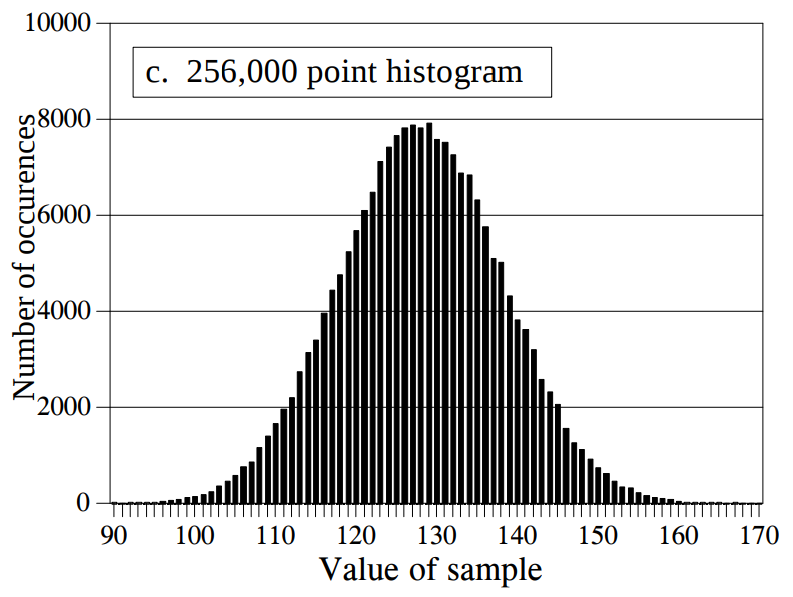
\includegraphics[width=0.45\textwidth]{figures/hist.png}
\caption{\label{fig:hist} The histogram contains counts versus sample values.}
\end{figure}
\end{frame}

\section{Conclusion}

\begin{frame}{Unit 0 Outline}
\begin{enumerate}
\item Topics from Chapter 1: 1.1, 1.2, 1.3
\begin{itemize}
\item What is a statistic?
\item Probability examples
\item Data and sampling
\end{itemize}
\item Topics from Chapter 2: 2.1 - 2.4, 2.5 - 2.8
\begin{itemize}
\item Data visualization
\item Location of the data in numerical space
\end{itemize}
\item Topics from Chapter 3: 3.1, 3.2, 3.3
\begin{itemize}
\item Two rules of probability
\end{itemize}
\end{enumerate}
\end{frame}

\end{document}
